\documentclass{book}
\usepackage{geometry}
\usepackage[utf8]{inputenc} % UTF-8 unterstützung
\geometry{papersize={170mm,240mm},total={140mm,200mm},top=21mm,bindingoffset=10mm}
\usepackage{ngerman}
\usepackage{times}
\usepackage{amsmath}
\usepackage{amssymb}
\usepackage{amsfonts}
\usepackage{amsthm}
\usepackage{graphicx}
\usepackage{fancyhdr}
\usepackage{textcomp}
\usepackage[all]{xy}
\usepackage{txfonts}
\usepackage{alltt}
\usepackage{verbatim}
\usepackage{paralist}
\usepackage{makeidx}
\usepackage{array}
\usepackage{hyperref}
\usepackage{listings}
\lstdefinestyle{Matlab}{
  numbers=left,
  belowcaptionskip=1\baselineskip,
  breaklines=true,
  frame=L,
  xleftmargin=\parindent,
  language=Matlab,
  showstringspaces=false,
  basicstyle=\footnotesize\ttfamily,
  keywordstyle=\bfseries\color{green!40!black},
  commentstyle=\itshape\color{purple!40!black},
  identifierstyle=\color{blue},
  stringstyle=\color{orange},
  numberstyle=\ttfamily\tiny
}
\usepackage{caption}
\usepackage{subcaption}
\usepackage{epstopdf}
\usepackage{standalone}
\usepackage[backend=bibtex]{biblatex}
\addbibresource{MonteCarlo.bib}



\begin{document}
\title{Monte Carlo Methode}
\author{Dorian Amiet, Hannes Badertscher}
\date{}
\maketitle



\chapter{Beispiel-Anwendung}
\rhead{Beispiel-Anwendung}
\begin{refsection}

\section{Einleitung}
Der Monte Carlo Algorithmus ist ein Verfahren zur Lösung numerischer Probleme durch das Ziehen von Zufallszahlen. Die Idee, mathematische bzw. physikalische Probleme mit einem stochastischen Sampling-Verfahren zu approximieren stammt polnisch-amerikanischen Mathematiker Stanisław Marcin Ulam (1909 -- 1984), welcher zu dieser Zeit im Los Alamos National Labaratory arbeitete. Seine Idee, und wie es dazu kam, beschrieb er folgendermassen: \\
 
\textit{“The first thoughts and attempts I made to practice [the Monte Carlo method] were suggested by a question which occurred to me in 1946 as I was convalescing from an illness and play- ing solitaires. The question was what are the chances that a Canfield solitaire laid out with 52 cards will come out successfully? After spending a lot of time trying to estimate them by pure combinatorial calculations, I wondered whether a more practical method than “abstract thinking” might not be to lay it out say one hundred times and simply observe and count the number of successful plays. This was already possible to envisage with the begin- ning of the new era of fast computers, and I immediately thought of problems of neutron diffusion and other questions of mathematical physics, and more generally how to change processes de- scribed by certain differential equations into an equivalent form interpretable as a succession of random operations. Later... [in 1946, I ] described the idea to John von Neumann and we began to plan actual calculations.”} - Stan Ulam, 1983 \\

Als erste Anwendung konnten Ulam und von Neumann mit der Monte Carlo Methode die Neutronen-Diffusion in spaltbaren Materialien simulieren. 

\subsection{Anwendungen}

Monte Carlo Methoden kommen überall zum Einsatz, wenn deterministische Algorithmen entweder zu komplex sind, oder gar nicht existieren. Dank zunehmender Rechenleistung sind in den letzten Jahren Simulationen wie globale Klimamodelle möglich geworden. Typische Anwendungen des Monte Carlo Algorithmus umfassen u.a.

\begin{itemize}
	\item Numerische Integration
	\item Simulation von dynamischen Prozessen
	\item Simulation von Gleichgewichtszuständen (z.B. mit Metropolis-Algorithmus)
	\item Statistische Untersuchung von Zufallsverteilungen
\end{itemize}


\section{Lösungsansatz}

\subsection{Zufallszahlengeneratoren}

Die Generierung von Zufallszahlen ist absolut essentiell für die Monte Carlo Methode. In der analogen Welt bestehen verschiedene hervorragende Zufallsgeneratoren, u.a. das thermische Widerstandsrauschen oder radioaktive Zerfallsvorgänge. So gab es in der Vergangenheit Ansätze, in welchen die Strahlung einer radioaktiven Quelle gemessen wurde und daraus eine Folge von Zufallszahlen generiert wurde. Heute werden eher Rauschgeneratoren mit Widerständen oder Dioden verwendet. In digitalen Schaltungen wird teilweise der Ausgang eines metastabilen Flip-Flop als Zufallszahlengenerator verwendet.\\

\subsection{Random-Device} \label{subsec:RandomDev}

Auf Unix-Systemen steht mit dem sog. Random-Device (/dev/random) ein Zufallszahlengenerator sehr hoher Güte zur Verfügung. Dieser sammelt das Rauschen von Gerätetreibern in einem Entropie-Pool und generiert daraus Zufallszahlen, welche auch höchsten Anforderungen im Bereich der Kryptografie genügen. Der Nachteil ist, dass sobald dieser Entropie-Pool erschöpft ist keine Zufallszahlen mehr generiert werden können. Mit dem Device /dev/urandom wurde Abhilfe geschaffen, was jedoch mit dem Nachteil erkauft wird, dass beim Unterschreiten einer gewissen Entropie-Schwelle nur Pseudozufallszahlen generiert werden, welche unter Umständen von einem potentiellen Angreifer berechnet werden könnten. Den meisten Anforderungen genügt dies jedoch trotzdem. \\

Das Random-Device kann von einem Programm wie ein File eingebunden werden und Zufallszahlen daraus gelesen werden. Für viele Anwendungen ist dies klar zu langsam, weshalb häufig das Random-Device nur als Seed für einen Pseudo-Random-Number-Generator verwendet wird.

\subsection{Multiplikativ kongruentielle Generatoren} \label{subsec:LCG}
Eine der populärsten Methoden zur Generierung von Zufallszahlen ist die multiplikativ kongruentielle Methode. Solche Generatoren werden häufig als \textit{linear congruential generator (LCG)} bezeichnet. Dabei werden Zufallszahlen rekursiv nach folgender Vorschrift berechnet:

\begin{equation}
	x_{i+1} = \left( a x_{i} + b \right) \, \text{mod} \, m
\end{equation}

Der Generator ist durch den Startwert $x_1$, den Faktor $a$, das Inkrement $b$ und das Modul $m$ vollständig bestimmt. Der grösste Nachteil der LCG-Generatoren ist die geringe Periode, sowie die eindeutige Korrelation von aufeinanderfolgenden Zufallszahlen, welche in Abbildung \ref{fig:lcg_verteilung} eindeutig sichtbar ist.

\begin{figure}[h]
	\centering
	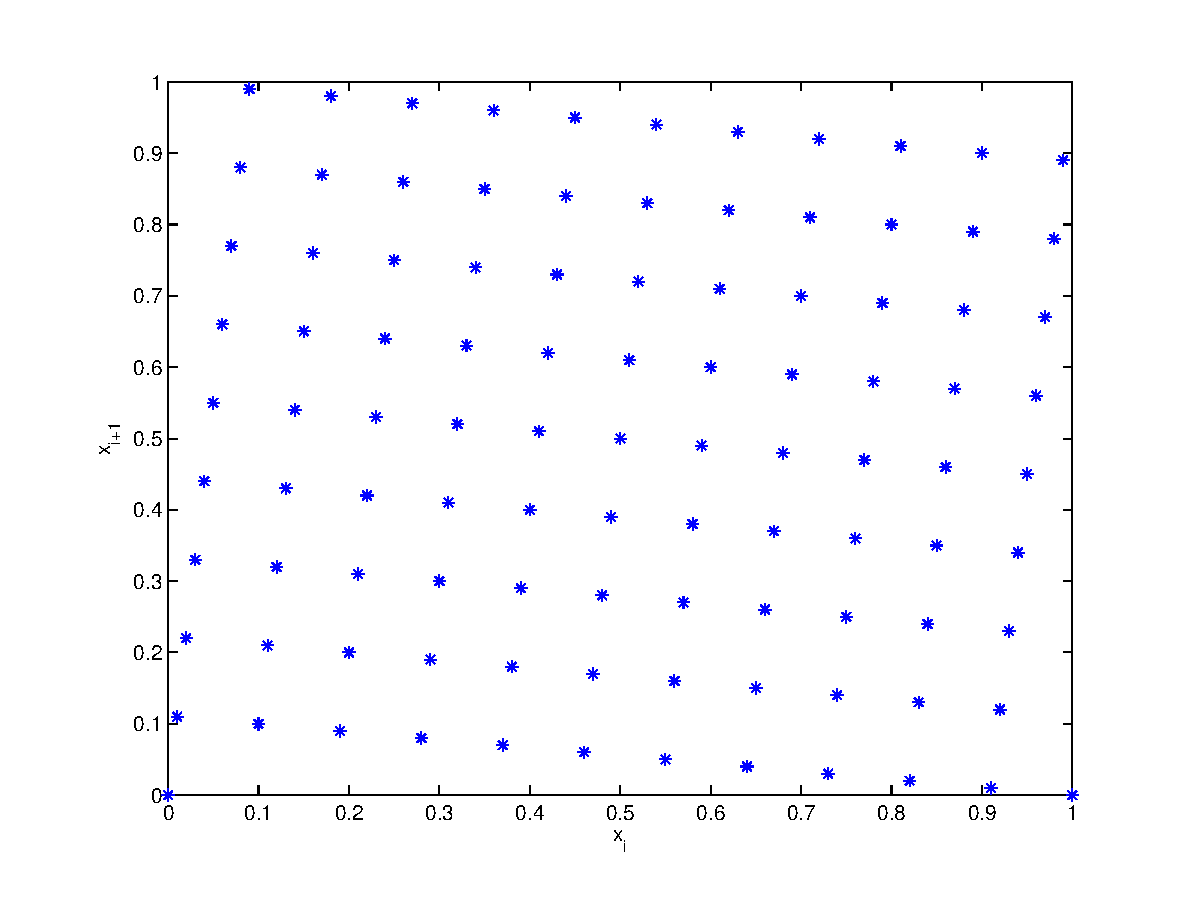
\includegraphics[width=8cm]{images/lcg.eps}
	\caption{Verteilung aufeinanderfolgender Zufallszahlen eines LCG mit $a=11$, $b=0$, $m=64$}
	\label{fig:lcg_verteilung}
\end{figure}

Durch die einfache Berechnung sind LCG Generatoren sehr verbreitet für Anwendungen, bei welchen keine hohen Anforderungen an die Zufallszahlen besteht. So verwendet die C-Funktion \textit{rand()} nach dem LCG-Algorithmus mit den Konstanten $a=1103515245$, $c=12345$, $m=2^{31}$, und dem mit der Funktion \textit{srand()} gesetzten Startwert. Häufig wird der Algorithmus mit der aktuellen Systemzeit initialisiert: \textit{srand( time(NULL) );}.

\subsection{Mersenne-Twister} \label{subsec:MersenneTwister}
Der Mersenne-Twister Algorithmus zeichnet sich durch eine extrem hohe Periode von $2^{19937}-1 \approx 4.3 \cdot 10^{6001}$ aus. Die Periodenlänge ist eine Mersenne-Primzahl\footnote{Mersenne-Primzahl: Primzahl der Form $2^{n}-1$} und gibt dem Algorithmus den Namen. Die Ausgabesequenz ist bis zur Dimension 623 gleichverteilt, d.h. werden die ausgegebenen Zahlen als Vektoren bis Dimension 623 interpretiert, so sind diese Vektoren immer gleichverteilt. \\

Der Mersenne-Twister Algorithmus arbeitet mit 624 Zustandswörtern $Y_1 \dots Y_N$ von typischerweise 32-bit Länge. Diese Zustände werden zu Beginn des Algorithmus initialisiert. Dies wird häufig mit dem in Abschnitt \ref{subsec:RandomDev} beschriebenen Random-Device oder mit einfacheren Zufallszahlgeneratoren wie dem LCG gemacht. Je besser (d.h. zufälliger) die Initialisierung, desto früher sind die generierten Zahlen auch zufällig. Ist dies nicht gewährleistet, kann $Y[2]$ mit einem zufälligen Seed, z.B. der Uhrzeit, initialisiert werden und $800'000$ Zahlen generiert werden, bevor der Algorithmus benutzt wird. So ist eine gute Gleichverteilung sichergestellt. \\

Der Algorithmus für alle darauf folgenden Zufallszahlen $Y_i$ für $i>N$ werden wie folgt berechnet:

\begin{align}
	h &:=  Y_{i-N} - Y_{i-N} \mod{2^{31}} + Y_{i-N+1} \mod{2^{31}} \\
	Y_i &:= Y_{i-227} \oplus \left\lfloor \frac{h}{2} \right\rfloor \oplus \left( \left(h \mod{2} \right) \cdot 9908b0df_{\text{hex}}\right)
\end{align}

Um sicherzustellen, dass alle 32-bit gleichverteilt sind, werden die Zufallszahlen $Z$ aus $Y$ wie folgt berechnet: 
\begin{align}
	x &:= Y_{i} \oplus \left\lfloor \frac{Y_i}{2^{11}} \right\rfloor \\
	y &:= x \oplus \left(\left(x \cdot 2^7\right) \wedge 9d2c5680_{\text{hex}} \right) \\
	z &:= y \oplus \left(\left(y \cdot 2^{15}\right) \wedge efc60000_{\text{hex}} \right) \\
	Z_i &:= z \oplus \left\lfloor \frac{z}{2^{18}} \right\rfloor
\end{align}

Obwohl der Mersenne-Twister Algorithmus sehr kompliziert scheint, ist die Ausführung relativ schnell. Zusammen mit den bereits beschriebenen Vorteilen hat dies dazu geführt, dass der Mersenne-Twister der Standard-Zufallszahlengenerator in vielen Bibliotheken, wie z.B. der \textit{GNU Scientific Library} ist.

\section{Implementationseigenheiten}
\section{Resultate}

\printbibliography[heading=subbibliography]
\end{refsection}

\end{document}